% !TEX root = ../thesis.tex
\chapter{Software Development Environment}\label{cha:software}
When just providing the hardware, the \gls{CPU} can hardly be used.
It is possible to write programs by hand by writing single bytes to the \glspl{EEPROM} that hold the program.
However, it is quite infeasible to write complex programs this way.
Even more extreme is content of the \glspl{EEPROM} holding the micro code, i.e. that decode the instruction depending on the instruction cycle and \gls{ALU} flags.

Therefore, the \gls{EDiC} comes with two main software utilities that form the Software Development Environment.

\section{Microcode Generation}\label{sec:microcode}
\begin{listing}[t]
  \inputminted[linenos,
    breaklines,
    frame=leftline,
    xleftmargin=20pt,
  ]{TypeScript}{src/microcode.ts}
  \caption{Schema of the Microcode Definition CSON-File \cite{CSON} as a TypeScript \cite{TS} Type definition.}
  \label{lst:micrcode_schema}
\end{listing}
The goal is to define all the available instructions and what they perform in which instruction step and then have a program automatically generate the bit-files for the \gls{EEPROM}.
This approach allows to easily make changes to the existing microcode if a bug was found or a new instruction should be added.
The file format which defines the microcode has to be human and machine readable as it should be easily edited by hand and also be read by the tool that generates the bit-files.
A very common file format for tasks like this is \gls{JSON} \cite{JSON} which is widely used in the computer industry.
Besides basic types as strings and numbers, it allows basic arrays with square brackets (\texttt{[]}) and objects with curly braces (\texttt{\{\}}).
Each object contains key value pairs and everything can be nested as desired.
For the \gls{EDiC} microcode generation \gls{CSON} was used which is very similar to \gls{JSON} but is slightly easier to write by hand because its syntax is changed a bit:
\begin{itemize}
  \item It allows comments which is extensively used to ease the understanding of individual instruction steps
  \item Braces and commas are not required
  \item Keys do not require string quotation marks
\end{itemize}
The schema for the file describing the microcode is shown in \cref{lst:micrcode_schema}.
The file is an object with three key, value pairs:
\paragraph{Signals}
\begin{listing}[h!]
  \begin{minted}[linenos,
    breaklines,
    frame=leftline,
    xleftmargin=20pt,
  ]{CoffeeScript}
  {
    name: 'reg0NWE'
    noOp: 1
  }
  \end{minted}
  \caption{Example of a control signal definition for the microcode generation.}
  \label{lst:mc_signals}
\end{listing}
The signals array consists of Objects that define the available control signals and the default value of the control signal.
\Cref{lst:mc_signals}
defines the \emph{not write enable signal for register 0} control signal and defines the default state as high.
This means, when this control signal is not specified it will stay high and, therefore, register 0 will not be written.

\paragraph{InstructionFetch} This array defines the steps that are performed at the beginning of each instruction to fetch the new instruction and decode it.
Each object represents one step and consists of key value pairs that define one control signal.
\begin{listing}[h!]
  \begin{minted}[linenos,
    breaklines,
    frame=leftline,
    xleftmargin=20pt,
  ]{CoffeeScript}
    instructionFetch: [
      { # write instruction
        memInstrNWE: 0
      }
      { # increment PC
        memPCNEn: 0
        memPCLoadN: 1
      }
    ]
  \end{minted}
  \caption{Definition of the instruction fetch and decode steps for the microcode generation.}
  \label{lst:mc_instrFetch}
\end{listing}

For example \cref{lst:mc_instrFetch} he first step specifies only the \emph{instruction not write enable} to be low and with this write the instruction into the instruction register.
Secondly, the \gls{PC} is incremented by setting \emph{PC not enable} to low and \emph{PC not load} to high.
\paragraph{Instructions} The instructions are an array of all available instructions.
Each instruction is defined as an \texttt{op} code, which is the 8 bit instruction in binary format.
However, if it was only possible to define the 8 bit as 0s and 1s instructions which only differ in the register used would need to be specified separately which is very error prone.
Therefore, it is allowed to specify the bit that specifies if register 0 or 1 is used to be set to \texttt{'r'} or \texttt{'s'} and then multiple instructions are generated.
Each instruction then The \texttt{cycles} array define the steps each instruction does in the same way as the \texttt{instructionFetch} array does.
However, as the value of individual control signals may depend up on which register is specified in the op code, it is also possible to specify \texttt{'r'}, \texttt{'!r'}, \texttt{'s'} or \texttt{'!s'}.

\begin{listing}[h!]
  \begin{minted}[linenos,
    breaklines,
    frame=leftline,
    xleftmargin=20pt,
  ]{CoffeeScript}
  {
    op: '1111100r' # r = imm
    cycles: [
      { # imm to bus to r
        reg0NWE: 'r'
        reg1NWE: '!r'
        memInstrNOE: 0
      }
    ]
  }
  \end{minted}
  \caption{Definition of the move immediate to register instruction for the microcode generation.}
  \label{lst:mc_movImm}
\end{listing}
\Cref{lst:mc_movImm} defines the move immediate to register instruction for both register at the same time.
The \emph{instruction immediate not output enable} is low and either register 0 or register 1 is written to.
This definition would be equal to \cref{lst:mc_movImmDuplicate}.
\begin{listing}[h!]
  \begin{minted}[linenos,
    breaklines,
    frame=leftline,
    xleftmargin=20pt,
  ]{CoffeeScript}
  [
    {
      op: '11111000' # r0 = imm
      cycles: [
        { # imm to bus to r0
          reg0NWE: 0
          reg1NWE: 1
          memInstrNOE: 0
        }
      ]
    }
    {
      op: '11111001' # r1 = imm
      cycles: [
        { # imm to bus to r1
          reg0NWE: 1
          reg1NWE: 0
          memInstrNOE: 0
        }
      ]
    }
  ]
  \end{minted}
  \caption{Definitions of the move immediate to register instruction for each register separately for the microcode generation.}
  \label{lst:mc_movImmDuplicate}
\end{listing}

This example is quite simple, however, instructions with two registers as arguments would result in four times the same definition and duplication can always result in inconsistencies.
The same idea is also used for the \gls{ALU} operations.
The \gls{ALU} operations are not generated by the microcode but are rather the three least significant bits of the instruction.
Therefore, all instructions using the \gls{ALU} can have the exact same control signals stored in the microcode \gls{EEPROM}.
To avoid 8 definitions of the same instructions, the op code can contain \texttt{'alu'} and all 8 instructions are generated.
\begin{listing}[h!]
  \begin{minted}[linenos,
    breaklines,
    frame=leftline,
    xleftmargin=20pt,
  ]{CoffeeScript}
  {
    op: '000rsalu' # r = r x s (alu)
    cycles: [
      { # r x s into alu
        aluYNWE: 0
        reg0BusNOE: 's'
        reg1BusNOE: '!s'
        regAluSel: 'r'
      }
      { # alu into r
        aluNOE: 0
        reg0NWE: 'r'
        reg1NWE: '!r'
      }
    ]
  }
  \end{minted}
  \caption{Definition of the alu operation with two register arguments for the microcode generation.}
  \label{lst:mc_aluRS}
\end{listing}
\Cref{lst:mc_aluRS} for example defines the alu operation with two registers and defines all 32 instructions with the op codes \texttt{'00000000'} to \texttt{'00011111'}.

\begin{listing}[h!]
  \begin{minted}[linenos,
    breaklines,
    frame=leftline,
    xleftmargin=20pt,
  ]{CoffeeScript}
  {
    op: '1010flag' # pc := imm
    cycles: [
      { # imm to pc
        memPCNEn: 0
        memPCLoadN: 0
        memPCFromImm: 1
      }
    ]
  }
  \end{minted}
  \caption{Definition of the branch instructions.}
  \label{lst:mc_branch}
\end{listing}
There is one final specialty built into the Microcode Generator:
The \gls{EDiC} has a branch instruction which is either executed or treated as a no-operation depending on the current state of the \gls{ALU} flags.
For all other instructions, the flags are ignored and always executed\footnote{Meaning that all memory locations for the instruction and step counter, no matter the \gls{ALU} flags, store the operation.}.
For this special instruction, the last for bits replaced with \texttt{flag} define at which state of the \gls{ALU} flags, the branch should be executed.
The possible conditions are heavily inspired by the conditional execution of ARM \glspl{CPU}\cite{armCond} as the \gls{ALU} flag architecture is very similar.
The possible values for the \texttt{flag} field and their meanings are listed in \cref{tab:mc_flagMeanings}.
Especially for a \gls{CPU} with only 8 bits it is important to support unsigned and signed operations and with a complex microcode it is no problem to support all the different branch instructions and with it facilitate the application design.
\begin{table}
  \centering
  \renewcommand{\arraystretch}{1.25}
  \caption{All available branch instructions with their op-code and microcode translation based on the \gls{ALU} flags explained in \cref{sec:alu}.}
  \label{tab:mc_flagMeanings}
  \begin{tabularx}{\textwidth}{ |c|l|l|X| }
    \hline
    \texttt{flag} (OP-Code) & Assembler Instruction                & \gls{ALU} flags                 & Interpretation   \\\hline\hline
    \texttt{0000}           & \texttt{jmp}/\texttt{bal}/\texttt{b} & Any                             & Always           \\\hline
    \texttt{0001}           & \texttt{beq}                         & \texttt{Z==1}                   & Equal            \\\hline
    \texttt{0010}           & \texttt{bne}                         & \texttt{Z==0}                   & Not Equal        \\\hline
    \texttt{0011}           & \texttt{bcs}/\texttt{bhs}            & \texttt{C==1}                   & Unsigned $\geq$  \\\hline
    \texttt{0100}           & \texttt{bcc}/\texttt{blo}            & \texttt{C==0}                   & Unsigned $<$     \\\hline
    \texttt{0101}           & \texttt{bmi}                         & \texttt{N==1}                   & Negative         \\\hline
    \texttt{0110}           & \texttt{bpl}                         & \texttt{N==0}                   & Positive or Zero \\\hline
    \texttt{0111}           & \texttt{bvs}                         & \texttt{V==1}                   & Overflow         \\\hline
    \texttt{1000}           & \texttt{bvc}                         & \texttt{V==0}                   & No overflow      \\\hline
    \texttt{1001}           & \texttt{bhi}                         & \texttt{C==1} and \texttt{Z==0} & Unsigned $>$     \\\hline
    \texttt{1010}           & \texttt{bls}                         & \texttt{C==0} or \texttt{Z==1}  & Unsigned $\leq$  \\\hline
    \texttt{1011}           & \texttt{bge}                         & \texttt{N==V}                   & Signed $\geq$    \\\hline
    \texttt{1100}           & \texttt{blt}                         & \texttt{N!=V}                   & Signed $<$       \\\hline
    \texttt{1101}           & \texttt{bgt}                         & \texttt{Z==0} and \texttt{N==V} & Signed $>$       \\\hline
    \texttt{1110}           & \texttt{ble}                         & \texttt{Z==0} or \texttt{N!=V}  & Signed $\leq$    \\\hline
    \texttt{1111}           & -                                    & Any                             & Never (Not used) \\\hline
  \end{tabularx}
\end{table}

\section{Assembler}
The second software that is probably even more important is the assembler.
An assembler translates human readable instructions into the machine code, i.e. the bits that are stored in the instruction \glspl{EEPROM}.
For the \gls{EDiC} each instruction is 24 bits wide, with 8 bits instruction op code and 8 or 16 bits immediate value.
Even though assemblers usually only translate instructions one for one, they can have quite advanced features.
With an assembler, the programmer is no longer required to know the specific op codes for all instructions and set individual bits of the instructions which is very error prone.
The assembler for the \gls{EDiC}, therefore, allows easier programming with a simple text-based assembly syntax similar to the well-known ARM syntax.
\begin{listing}
  \inputminted[linenos,
    breaklines,
    frame=leftline,
    xleftmargin=20pt,
  ]{ARM}{src/prng.s}
  \caption{\gls{PRNG} written in the \gls{EDiC} Assembler.}
  \label{lst:asm_prng}
\end{listing}

\begin{listing}
  \inputminted[linenos,
    breaklines,
    frame=leftline,
    xleftmargin=20pt,
  ]{ARM}{src/prng_out.s}
  \caption{The output of the \gls{PRNG} of \cref{lst:asm_prng}. The first 16 bits are the memory address, then 8 bits for the instruction op-code and 16 bits for the instruction immediate and for reference the original instruction with variables replaced.}
  \label{lst:asm_prng_out}
\end{listing}

\Cref{lst:asm_prng,lst:asm_prng_out} show the translation that the assembler does where \cref{lst:asm_prng} shows the assembler program that is written by any programmer and \cref{lst:asm_prng_out} summarizes what values are stored in the program \gls{EEPROM}.

\subsection{Calling conventions}
Even though calling conventions are strictly speaking not a feature of the assembler, it is an important factor to keep in mind with functional programming.
Calling conventions are a set of rules which caller (the instructions calling a subroutine) and callee (the subroutine that is called) should usually follow.
\paragraph{Parameters}
Usually the first parameters from the caller to the callee are passed in registers, which avoids long memory operations for storing and loading the parameters.
In the \gls{EDiC} memory operations cannot stall and are, therefore, not slower than register operation and the \gls{EDiC} has only 2 registers.
Therefore, only the very first argument is passed in \texttt{r0} and all further arguments are passed in the memory.
The parameters are stored on the stack of the callee starting at stack address \texttt{0x00} (\texttt{0xff00} as memory address).
\paragraph{Return value}
The return value is to be place in \texttt{r0}.
If a return value larger than 8 bit (or multiple 8 bit values) are to be returned, the caller may pass a pointer to a memory location as a parameter and the callee works on the memory content pointed to.
\paragraph{Preservation}
The register \texttt{r1} can to be used as a function local variable and, therefore, has to be preserved by any callee.
This is usually done by storing the content on the stack at the beginning of the function and restoring them from the stack at the end of the function.

\subsection{Available Instructions}
First of all, this section summarizes all available instructions and which parameters they take.
All instructions start with the operation and then up two parameters separated by a comma.

There are four different parameter types.
It can either be a register specified as \texttt{r0} or \texttt{r1}.
The register value can also be passed as the address to a memory operation with \texttt{[r0]}.

Immediate values can also be specified as value or as address with brackets around the immediate value.
However, the syntax for immediate values is more complex, as the assembler can parse decimal (positive and negative) as well as hexadecimal numbers.
Additionally, variables can be used which are further explained in \cref{sec:constants}.

When specifying a value, the immediate can range between -127 and 255 (two's complement and unsigned) and when used as an address it can range between 0 and 0xfffe (65534). The upper limit is not 0xffff because that address is reserved for the return address and should not be overwritten.
\subsubsection{\gls{ALU} Instructions}
The following \gls{ALU} instructions are available:
\begin{multicols}{4}
  \begin{itemize}
    \item add
    \item sub
    \item and
    \item eor
    \item xor
    \item xnor
    \item lsr
    \item lsl
  \end{itemize}
\end{multicols}
\gls{ALU} instructions always take two parameters. The first parameter is the left hand side operand and the register where the result is stored in and the second parameter is the right hand side operand.
\begin{itemize}
  \item Two registers

        \qquad\mintinline{ARM}{sub r0, r1} does: $r_0:=r_0-r_1$
  \item One register and one register as memory address

        \qquad\mintinline{ARM}{lsr r1, [r0]} does: $r_1:=r_1\gg\text{mem}[r_0]$ (\cref{sec:memInstr})
  \item One register and an immediate value

        \qquad\mintinline{ARM}{and r0, 0x0f} does: $r_0:=r_0\xor 15$
  \item One register and an immediate value as memory address

        \qquad\mintinline{ARM}{add r1, [0x0542]} does: $r_1:=r_1+\text{mem}[1346]$
\end{itemize}
All of the \gls{ALU} instructions can have an `s' as suffix which has the effect that the result of the operation is not written to the first operand.
This is useful when a calculation is only performed to update the \gls{ALU} flags but the register value is used later on.
This results in a special \gls{ALU} instruction: \mintinline{ARM}{cmp} which is an alias to \mintinline{ARM}{subs} which is typically used to compare to values and perform a branch instruction based on the result.
\begin{minted}{ARM}
cmp r0, 10 // equal to subs r0, 10
blt 0x42
\end{minted}
compares the \texttt{r0} register with the value 10 and if $r0 < 10$ branches to instruction at address 66 and preserves the content of \texttt{r0}.

\subsubsection{Memory Instructions}\label{sec:memInstr}
The following memory instructions are supported:
\begin{multicols}{4}
  \begin{itemize}
    \item str
    \item ldr
    \item sts
    \item lds
    \item stf
    \item ldf
    \item sma
  \end{itemize}
\end{multicols}

The two common instructions are \mintinline{ARM}{str} and \mintinline{ARM}{ldr} which are \emph{store} and \emph{load} operations.
These two instructions take two parameters:
Th first is the register used in the store or load operation and the second is the memory address.
They either take an 16bit immediate address which is used as the full address for the access or a register as address.
As the registers are only 8 bits, the register value is only used for the lower 8 bits of the address and the upper 8 bits are the value of the \gls{MAR}.
The upper 8 bits of the \gls{MAR} can be set with the \mintinline{ARM}{sma} instruction which takes either a register or an 8 bit immediate value.

The \mintinline{ARM}{lds} and \mintinline{ARM}{sts} instructions are used for accessing the stack.
They only take immediate addresses and the compile makes sure that the addresses upper 8 bits are \texttt{0xff} to always access the stack.

The \mintinline{ARM}{ldf} and \mintinline{ARM}{stf} functions work very similar in only accessing the stack.
However, before the memory access, the \gls{SP} is incremented and after the access, it is restored.
This way, it is possible to access parameters of a function that is called.

Some examples:

\begin{tabular}{m{.3\textwidth}m{.65\textwidth}}
  \mintinline{ARM}{ldr r0, [0xabba]} & Loads the value from address \texttt{0xabba} into \texttt{r0}                                                                       \\
  \mintinline{ARM}{str r1, [0xc0de]} & Stores the value in \texttt{r1} to address \texttt{0xc0de}                                                                          \\
  \begin{minted}{ARM}
sma 0xca
mov r0, 0xfe
ldr r0, [r0]
  \end{minted}
                                     & Loads the value from address \texttt{0xcafe} into \texttt{r0}                                                                       \\
  \mintinline{ARM}{lds r1, [0x42]}   & Loads the value fromm address \texttt{0xff42} which is translated into \texttt{0x\{sp\}42} into \texttt{r1}                         \\
  \mintinline{ARM}{stf r0, [0xab]}   & Stores the value in \texttt{r0} to address \texttt{0xffab} with incremented \gls{SP} which is translated into \texttt{0x\{sp+1\}ab} \\
\end{tabular}

\subsubsection{Miscellaneous Instructions}
There are four more instructions that are essential:

\begin{multicols}{4}
  \begin{itemize}
    \item mov
    \item b
    \item call
    \item ret
  \end{itemize}
\end{multicols}
The \mintinline{ARM}{mov} instruction either takes two registers or one register and an 8 bit immediate value as parameters.
When specifying two registers, the content of the second register is copied to the first register.
Otherwise, the immediate value is stored in the register.
The branch (\mintinline{ARM}{b}) instruction takes a 16 bit immediate value which is used as the new \gls{PC} content.
It is the only conditional instruction that is available in the \gls{EDiC} instruction set.
The second column of \cref{tab:mc_flagMeanings} lists all the possible suffixes for conditional branches and their meanings.
If the condition is met, the branch is executed, otherwise the instruction has no effect.

The \mintinline{ARM}{call} instruction also takes a 16 bit immediate address which is the destination address for the call.
In contrast to the branch instruction, the call is not conditional (i.e. it is always executed) and has the side effect of incrementing the \gls{SP} and storing the current \gls{PC} on the stack at address \texttt{0x\{sp\}ff}.

The \mintinline{ARM}{ret} instruction is used at the end of a function without any parameters to restore the \gls{PC} from the stack at address \texttt{0x\{sp\}ff} and decrement the \gls{SP} again.

Some examples:

\begin{tabular}{m{.3\textwidth}m{.65\textwidth}}
  \mintinline{ARM}{mov r0, 0xda} & Sets \texttt{r0} to \texttt{0xda}                                                                       \\
  \mintinline{ARM}{mov r1, r0}   & Copies the value of \texttt{r0} to \texttt{r1}                                                          \\
  \begin{minted}{ARM}
cmp r0, 10
blt 0x42
  \end{minted}
                                 & Branches to address (sets the \gls{PC} to) \texttt{0x42} if the value of \texttt{r0} is smaller than 10 \\
  \mintinline{ARM}{call 0x100}   & Calls a function at address \texttt{0x100}                                                              \\
  \mintinline{ARM}{ret}          & Returns from a function to the caller
\end{tabular}

\subsection{Constants}\label{sec:constants}
One main improvement that an assembler allows over manually setting the instruction bits is the use of constants in the code.
They can be declared to represent a value and then used similarly to variables of higher level languages instead of hard coded numbers.
The \gls{EDiC} assembler supports three kinds of constants: Value constants, labels and string constants.
\subsubsection{Value constants}\label{sec:vconstants}
Value constants are the easiest kind of constants available.
The first two lines of \cref{lst:asm_prng,lst:asm_prng_cmp} both declare a common constant that is used exactly like in higher level languages.
Each instruction, taken an immediate value can instead specify the name of the constant and the value of the constant is then used instead.
In \cref{lst:asm_prng_cmp} line 5 (\mintinline{ARM}{ldr r0, [PRNG_SEED]}) is assembled into the same instruction as \mintinline{ARM}{ldr r0, [0x00]}.
Constant declarations have the format \texttt{<name> = <value>}.

These value constants can be used to make the code easier to understand.
For example \mintinline{ARM}{str r0, [SIMPLE_IO]} makes it clearer that the value of r0 is not stored in some memory location but rather send to some I/O device (in this case the internal I/O register from \cref{sec:IO}).
It also prevents errors where a typo in an address causes unintended behavior of the code.

\subsubsection{Labels}
\begin{listing}
  \begin{multicols}{2}
    \inputminted[linenos,
      breaklines,
      frame=leftline,
      xleftmargin=20pt,
    ]{ARM}{src/prng.s}
    \inputminted[breaklines, frame=leftline]{ARM}{src/prng_cmp.s}

  \end{multicols}
  \caption{The \gls{PRNG} of \cref{lst:asm_prng} with the constants and labels resolved.}
  \label{lst:asm_prng_cmp}
\end{listing}
Instruction labels are often used in assemblers are a huge convenience.
They are declared by specifying a label name followed by a colon and hold the address of the next instruction.
Then, they can be used as immediate values for branch and call instructions to jump to the instruction followed by the label declarations.
As seen in \cref{lst:asm_prng} the line 21 (\mintinline{ARM}{call prng}) is assembled into the instruction \mintinline{ARM}{call 0x01} which is the location of the instruction after the declarations of the \texttt{prng} label (\mintinline{ARM}{ldr r0, [PRNG_SEED]}).

The load instruction from line 5 is actually the first instruction of the \gls{PRNG} algorithm, however, it is not assembled as the first instruction.
This is due to a special label being declared in the code at line 17.
When the \texttt{start} label is declared, then a new instruction is inserted at the beginning which unconditionally branches to the instruction after the start label.
This can be seen in \cref{lst:asm_prng_out} where the first instruction is a \mintinline{ARM}{b 0x0a} because the first instruction after the start label got assembled to the address \texttt{0x0a}.
The use of the start label comes especially clear in the \cref{sec:imports}.

\subsubsection{String constants}
\begin{listing}
  \inputminted[linenos,
    breaklines,
    frame=leftline,
    xleftmargin=20pt,
  ]{ARM}{src/snake_excerpt.s}
  \caption{Excerpts of the Snake assembler program used in the demo in \cref{fig:EDiCSnake}.}
  \label{lst:asm_snake_excerpt}
\end{listing}


The third constant is rather advanced and uses very \gls{EDiC} specific features.
It allows the definition of character strings with a maximum length of 255 chars which can later be used.
Differently to the value constants of \cref{sec:vconstants} strings cannot be used as parameters to instructions directly, because a string is a rather complex data structured in the context of assemblers.
In the \gls{EDiC} assembler a string can be defined as shown in \cref{lst:asm_snake_excerpt} line 4 with the syntax \texttt{<address>.<name> = "<value>"}.
In the example a string constant with the name ``LOST\_STRING'' is defined to have the content ``You lost!!! Score: '' at the address \texttt{0x20}.
The \gls{EDiC} assembler treats a string as an NULL-terminated array of characters which are characters stored consecutively and after the last character a NULL-byte is stored to signal the end of the string.
The address of a string constant actually defines the upper 8 bits of the address where the string is stored and is also the value of the constant itself.
This means that the string in the example is actually stored at addresses \texttt{0x2000} to \texttt{0x2013} (18 characters plus 1 NULL-byte) and \mintinline{ARM}{mov r0, LOST_STRING} in line 9 is equivalent to \mintinline{ARM}{mov r0, 0x20}.
As the assembler has no direct control over the memory contents as for example the ARM assembler, each string declarations results in two instructions per character that are inserted at the start of the program\footnote{Before the \mintinline{ARM}{b start} instruction that is inserted when a start label exists.} as shown in \cref{lst:asm_string_out}.

\begin{listing}[t]
  \begin{multicols}{2}
    \inputminted[linenos,
      breaklines,
      % firstline=1,
      lastline=21,
      frame=leftline,
      xleftmargin=20pt,
    ]{ARM}{src/snake_excerpt_str.s}
    \inputminted[linenos,
      breaklines,
      firstline=22,
      % lastline=21,
      frame=leftline,
      xleftmargin=20pt,
    ]{ARM}{src/snake_excerpt_str.s}

  \end{multicols}
  \caption{The instructions resulting from the string definition of \cref{lst:asm_snake_excerpt} line 4.}
  \label{lst:asm_string_out}
\end{listing}
\Cref*{lst:asm_snake_excerpt} lines 15 to 31 show a function that gets the upper 8 bits of the string address as a parameter in \texttt{r0}.
It outputs the characters one by one in a loop until the NULL-byte is reached.
To retrieve each character, firstly the \mintinline{ARM}{sma} instruction is called with the \glspl{MSB} of the address and then the \mintinline{ARM}{ldr} instruction with the loop register \texttt{r1} as an address argument is called.
The character (in \texttt{r0}) is then passed as an argument to the \texttt{uart\_write} function.

\subsection{File imports}\label{sec:imports}
An important factor of software development is reusability.
This also holds for assembler development and is the reason why the \gls{EDiC} assembler supports including other assembler files.
This can for example be used to write a library utility and then importing its functions for multiple projects.
This way, a bug fix in the utility library will be fixed across all projects at the same time.

As can be seen in \cref{lst:asm_snake_excerpt} lines 1 and 2, the \gls{EDiC} assembler supports the \texttt{include} keyword followed by a relative filename in double quotes.
Before assembling a file, all the include statements are replaced with the content of the file specified.
All the constants and labels are used as is with some exceptions:
\begin{itemize}
  \item The start label of all included files are discarded and the main file is required to provide a start label.
  Otherwise, the starting point is ambiguous and probably not where the programmer expects it.
  \item Constants from included files can be overwritten in the main file.
  This can be useful when value constants hold memory locations of global variables that need to be repositioned in the main file.
\end{itemize}


\subsection{Syntax Definition for VS Code}
\begin{figure}[t]
  \centering
  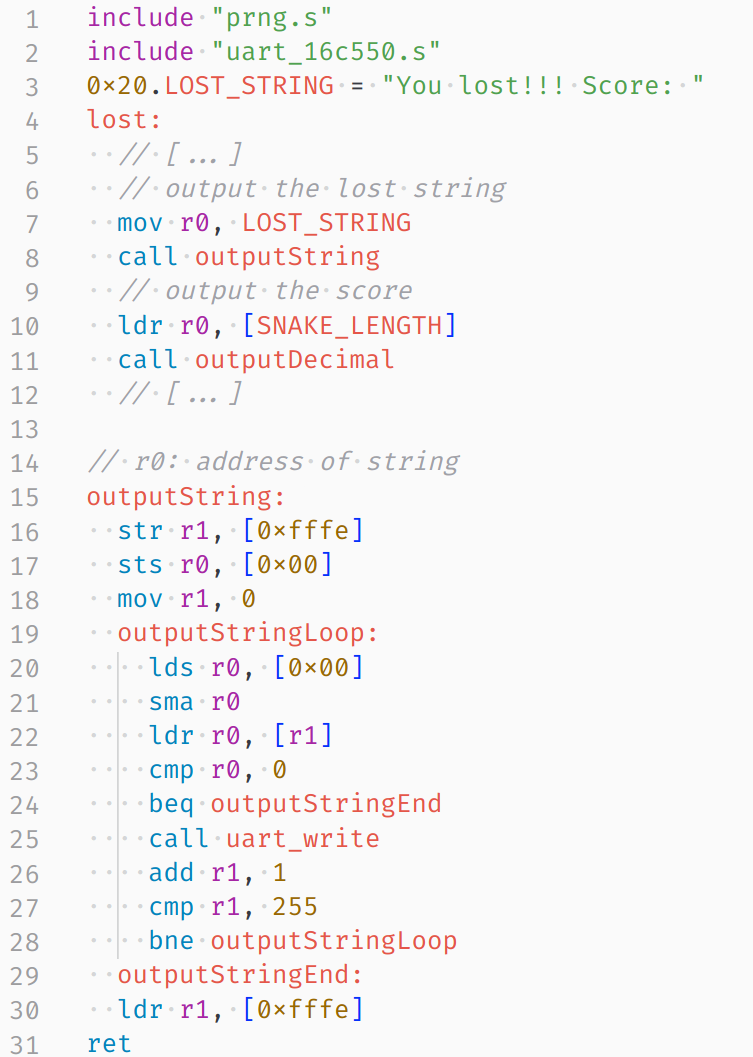
\includegraphics[width=.7\textwidth]{syntax_snake_excerpt.png}
  \caption{The syntax highlighting with the \gls{EDiC} Visual Studio Code Extension and the Atom One Light Theme \cite{VSCodeLight}.}
  \label{fig:SyntaxEDiC}
\end{figure}
Syntax Highlighting has become a very important factor for software development as \glspl{IDE} grow more capable.
The highlighting is usually done by firstly, parsing the syntax and associating parts of the text file with specific categories and, secondly, assigning styles like font color to these categories.
This way, a programmer can select a global color scheme which will define colors for different categories for all programming languages.
When applied correctly, code in different languages becomes easier to recognize because variables are always colored the same way, no matter the language.
The syntax parser, however, needs to be selected correctly for each file type and categorize the file content correctly.

Even though the \gls{EDiC} syntax is similar to the ARM syntax, it is not syntactically identical which makes syntax highlighting in editors difficult.
As can be seen in \cref{lst:asm_snake_excerpt} line 3, the ARM syntax definition used for the highlighting in this document is not perfect (The leading 0 is red and the string is not colored correctly).

As Visual Studio Code \cite{VSCode} is one of the leading extensible code editors, an extension for \gls{EDiC} assembler has been developed and published \cite{VSCodeEDiC}.
The code of the \cref{lst:asm_snake_excerpt} is shown again in \cref{fig:SyntaxEDiC} as it is highlighting using the developed extension.
The extension itself mainly consists of a TextMate language definition \cite{TextMate} and configuration files to work correctly with Visual Studio Code.
TextMate is a tokenization engine which works with a structured collection of regular expressions as language definitions.